\section{Anillos de enteros cuadráticos}

\begin{definition}
Para cada $n \in \mathbb{Z}$ que no sea un cuadrado perfecto, se define el conjunto de los enteros cuadráticos de radicando n como $\mathbb{Z}[\sqrt{n}] = \{a+b\sqrt{n}:a,b \in \mathbb{Z}\}$.

A este conjunto se le dota de estructura de anillo mediante las operaciones:

\begin{itemize}
\item Suma: $(a+b\sqrt{n})+(c+d\sqrt{n}) = (a+c) + (b+d)\sqrt{n}$
\item Producto: $(a+b\sqrt{n}) \cdot (c+d\sqrt{n}) = (ac+bdn)+(ad+bc)\sqrt{n}$
\end{itemize}

Dado un entero cuadrático $x = a + b \sqrt{n} \in \mathbb{Z}[\sqrt{n}]$ definimos su conjugado $\overline{x} = a - b \sqrt{n}$ y su norma como $N(x) = x \overline{x} = a^2-nb^2$. 
\end{definition}

\begin{proposition}
1. $\mathbb{Z} \subseteq \mathbb{Z}[\sqrt{n}] \land \mathbb{Z} = \mathbb{Z}[\sqrt{n}] \iff n$ es un cuadrado perfecto. \\
2. $\mathbb{Z}[\sqrt{n}]$ es un subanillo de $\mathbb{C}$ y si $n > 0$ entonces $\mathbb{Z}[\sqrt{n}]$ es un subanillo de $\mathbb{R}$. \\
3. $-:\mathbb{Z}[\sqrt{n}] \to \mathbb{Z}[\sqrt{n}]$ es un homomorfismo idempotente.\\
4. $N:\mathbb{Z}[\sqrt{n}] \to \mathbb{Z}$ es un homomorfismo de anillos.\\
5. $U(\mathbb{Z}[\sqrt{n}]) = \{x: N(x) \in \{1, -1\}\}$. 
\end{proposition}
\begin{proof}
1. Trivial.

2. Basta comprobar que la suma y el producto son cerradas en $\mathbb{Z}[\sqrt{n}]$ y se corresponden con las operaciones de los complejos. También se verifica que $1,-1 \in \mathbb{Z}[\sqrt{n}]$ de donde se tiene que es un subanillo de los complejos. La otra propiedad es entonces trivial. 

3. Si $x = (a,b) \land y = (c,d)$ entonces $\overline{x+y} = \overline{(a+c,b+d)} = \overline{(a+c,-b-d)} = (a,-b) + (c,-d) = \overline{x} + \overline{y}$. Análogamente se procede para el producto. Finalmente, $\overline{\overline{x}} = \overline{(a,-b)} = x$. 

4. $N(xy) = (xy)(\overline{xy}) = xy\overline{x}\overline{y} = x \overline{x} y \overline{y}$. Por otro lado, $N(xy) = N(x)N(y) = N(y)N(x)$ y finalmente, $N(1) = 1^2-0n = 1$. Hemos usado varias veces que el producto es commutativo por tratarse de un subanillo de $\mathbb{C}$. 

5. $\subseteq)$ Como $N$ es un homomorfismo, preserva las unidades y por tanto, si $x \in U(\mathbb{Z}[\sqrt{n}] \implies x \in U(\mathbb{Z}) = \{1,-1\}$.

$\supseteq)$ Observemos que $N(x) = x\overline{x}$. Si $N(x) = 1$ entonces $x^{-1} = \overline{x}$ y si $N(x) = -1$ entonces  $x^{-1} = - \overline{x}$. Luego en cualquier caso tenemos una unidad del anillo.  
\end{proof}

\begin{example}
El anillo de los enteros de Gauss es $\mathbb{Z}[i] = \{a+bi:a,b \in \mathbb{Z}\}$. Está claro que en este anillo $N(a+bi) = a^2 + b^2$ y las soluciones de $N(a+bi) = 1 \lor N(a+bi) = -1$ son las parejas $(a,b)$ de la forma $(0,1),(0,-1),(1,0),(-1,0)$. Por tanto, $U(\mathbb{Z}[i]) = \{1,-1,i,-i\}$. 

\begin{figure}[H]
\centering
\makebox[\textwidth][c]{
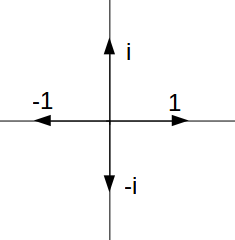
\includegraphics[scale=0.5]{./images/roots.png}
}
\end{figure}

El anillo de los enteros cuadráticos de radicando 2 es $\mathbb{Z}[\sqrt{2}] = \{a+b\sqrt{2}:a,b \in \mathbb{Z}\}$. Este anillo tiene como unidades todas las soluciones $(a,b)$ de las ecuaciones $a^2-2b^2 = 1 \lor a^2-2b^2 = -1$. Obsérvese que como $N(1+ \sqrt{2}) = -1$ entonces $N((1+\sqrt{2})^k = (-1)^k$ y por tanto todo $(1+\sqrt{2})^k$ son unidades del anillo. Se puede demostrar que todas las unidades del anillo son de esta forma. 

\end{example}

\section{Cuerpo de racionales cuadráticos}

\begin{definition}
Para cada $n \in \mathbb{Z}$ que no sea un cuadrado perfecto, se define el conjunto de los racionales cuadráticos de radicando n como $\mathbb{Q}[\sqrt{n}] = \{a+b\sqrt{n}:a,b \in \mathbb{Q}\}$.

A este conjunto se le dota de estructura de anillo mediante las operaciones:

\begin{itemize}
\item Suma: $(a+b\sqrt{n})+(c+d\sqrt{n}) = (a+c) + (b+d)\sqrt{n}$
\item Producto: $(a+b\sqrt{n}) \cdot (c+d\sqrt{n}) = (ac+bdn)+(ad+bc)\sqrt{n}$
\end{itemize}

Dado un racional cuadrático $x = a + b \sqrt{n} \in \mathbb{Q}[\sqrt{n}]$ definimos su conjugado $\overline{x} = a - b \sqrt{n}$ y su norma como $N(x) = x \overline{x} = a^2-nb^2$. 
\end{definition}

\begin{proposition}
1. $\mathbb{Q}$ es un subcuerpo de $\mathbb{Q}[\sqrt{n}]$ y $\mathbb{Q}[\sqrt{n}]$ es un subanillo de $\mathbb{C}$.\\
2. $-:\mathbb{Q}[\sqrt{n}] \to \mathbb{Q}[\sqrt{n}]$ es un homomorfismo idempotente.\\
3. $N:\mathbb{Q}[\sqrt{n}] \to \mathbb{Q}$ es un homomorfismo de anillos.\\
4. $\mathbb{Q}[\sqrt{n}]$ es el cuerpo de fracciones de $\mathbb{Z}(\sqrt{n})$. 
\end{proposition}
\begin{proof}
1. Trivial. 

2.3. La demostración es la misma que en el caso de los enteros cuadráticos. Nótese sin embargo la diferencia entre los codominios de las aplicaciones norma y conjugado. 

4. Basta ver que todo elemento no nulo admite un inverso. Para ello consideremos que $N(x) = x \overline{x}$ no es nulo salvo que $x$ sea nulo ya que en otro $n$ sería un cuadrado perfecto. Podemos por tanto definir $x^{-1} = \frac{\overline{x}}{N(x)}$ y se tiene que los racionales cuadráticos forman un cuerpo. 
\end{proof}